\documentclass[11pt]{article}

\usepackage[utf8]{inputenc}
\usepackage[scale=0.75,a4paper]{geometry}
\usepackage[german]{babel}
\usepackage{verbatim}
\usepackage{hyperref}
\usepackage{pgfplots} % LaTeX
\usepackage{graphicx}
\usepackage{tabularx}


%opening
\title{InformatiCup - Dokumentation}
\author{Tilman Hinnerichs, Tobias John}

\begin{document}

\maketitle

\begin{abstract}
	Im Folgenden soll unsere Lösung der Aufgaben des 13. InformatiCup 2018 vorgestellt werden. Dabei möchten wir unsere Annahmen zur Aufgabenstellung, unsere Lösung für beide Probleme und deren Bewertung, und einen Ausblick unserer Lösung beschreiben und erklären.  
\end{abstract}

\section{Annahmen zur Aufgabenstellung und Umformungen der Eingabedaten}
	Für Umsetzung unserer Lösung mussten wir dafür sorgen, dass die Werte nicht nur eingelesen, sondern auch so umgeformt werden, dass diese bestimmte Kriterien erfüllen.  
\subsection{Umformung der Tankstellendaten}
	Die Datei der Tankstellendaten stellt sehr viele unterschiedliche Daten zur Verfügung. Die reichen von der ID der Tankstelle, über die Postleitzahl zu den Koordinaten der Tankstelle. Für unser Verfahren ist sind folgende Kriterien wichtig: \\
	\begin{enumerate}
		\item \textbf{Individualität} der Tankstellen um diese eindeutig zuordnen und um über diese in einer Liste iterieren zu können
		\item \textbf{Örtliche Zuordnung} der Tankstellen um zwischen ihnen Abstände zu errechnen
	\end{enumerate} 
	Um eventuell später Zusammenhänge einzubeziehen oder wiederzuerkennen, haben wir zusätzlich die Marke der einzelnen Tankstellen mit einbezogen. Dies bildet aber zur Erfüllung der obigen Kriterien keinen Mehrwert. \\
	So werden bei der Einbeziehung der Tankstellendaten nur deren ID, Marke und Koordinaten aus den Tankstellendaten aus oben genannten Gründen herausgelesen. 
\subsection{Umformung der historischen Benzinpreisdaten}
	Die Daten, die wohl am wichtigsten für die Voraussage der Benzinpreise selbst sind, sind die historischen Tankstellendaten. Bei diesen stehen Tausende von Daten pro Tankstelle zur Verfügung. Pro Änderung des Benzinpreises stehen dabei das Datum mit der Uhrzeit mit einer Genauigkeit bis auf die Sekunde genau und der zugehörige neue E5-Benzinpreis zur Verfügung. 
	\\
	Kriterien für die Umformung dieser Daten sind die folgenden:
	\begin{enumerate}
		\item \textbf{Vergleichbarkeit} der Datensätze um mit ihnen eine Einteilung in bestimmte Kategorien vorzunehmen
		\item \textbf{Kontinuität} der Daten um eine Vergleichbarkeit der Daten bestimmter gleicher Intervalle zu erreichen und um diese in Algorithmen einfüttern zu können
		\item \textbf{Diskretisierung} der gemessenen Zeitpunkte
		\item \textbf{Handhabbare Menge} an Daten um mit ihnen noch in annehmbarer Zeit rechnen zu können, aber ebenfalls noch so viel, dass nicht zu viel Information verloren geht
	\end{enumerate}

	Um eine Vergleichbarkeit der Datensätze zu gewährleisten mussten wir die Kontinuität der Daten erreichen. Dazu rundeten wir jeden der Änderungszeitpunkte auf seine Stunde herunter und rechneten dabei ebenfalls die zugehörige Zeitverschiebung mit ein. Ebenfalls reicherten wir die Daten mit den Preisen zwischen diesen Änderungszeitpunkten an. Was auf den ersten Blick recht trivial wirkt, nimmt bei weiteren Algorithmen sehr viel Arbeit ab. So beträgt beispielsweise der Benzinpreise nach einer Änderung auf ein bestimmtes Niveau bis zu seiner nächsten Änderung diesen Wert bei. Durch diese Anreicherung besteht ein jeder Tag von Werten in der Geschichte einer Tankstelle aus 24 Werten. Dies bietet ebenfalls eine wunderbare Unabhängigkeit von schnell schwankenden Preisen innerhalb eines Tages und eben die oben gewünschte Vergleichbarkeit, da nun die Werte eines Tages mit 24 Werten dargestellt werden können. Damit ist zugleich die Kontinuität durch die gleichen Intervalle zwischen den Messpunkten und die Diskretisierung durch 24 feste Punkte innerhalb der sonst linearen Zeit gegeben. \\ Abschließend ist aus unserer Sicht das dilemmaartige vierte Kriterium der handhabbaren Menge an Daten gewährleistet. So sind durch die Einteilung noch eine Menge von $ 24 * 365 * 3 = 26.280 $ Werten (bei ca. 3 betrachteten Jahren der historischen Tankstellenwerte) vorhanden, was eine ausreichende Genauigkeit für zukünftige Voraussagen mit unserer Methode bietet und eine für Computer komfortable Anzahl an Werte bildet.
		
\subsection{Umformung der Routendaten}
	Die Routendaten sind vor allem für die Berechnung der besten Route von Bedeutung. Diese enthalten neben der maximalen Tankkapazität des Fahrzeugs auch die Ankunftszeiten an den bestimmten Tankstellen, sowie deren ID. Um hier die Kausalität der bisherigen Daten weiterzuführen, diskretisieren wir wieder die Daten auf die volle Stunde und verwerfen für unser Modell zu spezifische  Daten wie Minuten und Sekunden. Weitere Annahmen müssen dabei für die Routendaten nicht getätigt werden, um sie in Konformität zu bringen.
\subsection{Umformung der Preisvorhersagedaten}
	Die getätigten Annahmen zu den Preisvorhersagedaten sind ähnlichen zu den unter \glqq Umformung der Routendaten\grqq{} getätigten Annahmen. So wird wieder sowohl der Zeitpunkt, welcher als zuletzt bekannt angenommen werden soll, als auch der Zeitpunkt, bis zu welchem die Vorhersage reichen soll, auf die jeweilige Stunde gerundet, um in das oben angerissene Datenmodell zu passen.



\section{Algorithmenidee}
\subsection{Lösung der Benzinpreis-Vorhersage-Problems}
\subsubsection{Ansatz}
	%Welche Algorithmen wurde hier benutzt uns was versprechen wir uns davon? Warum haben wir das ganze in Intervalle unterteilt? Gehen wir auf etwaige Sonderdaten wie in der Aufgabenstellung genannt ein (Schulferien, Adresse,) 
	
	\paragraph{Annahmen\\}
	Unsere Vorhersagemodell beruht auf zwei simplen Annahmen: 
	\begin{enumerate}
		\item Die Preise folgen \textbf{sich wiederholenden Mustern}, d.h. die aktuelle Preisentwicklung wird sich fortführen, wie es ähnliche Entwicklungen in der Vergangenheit getan haben. Folgte z.B. in der Vergangenheit auf drei Tage starken Preisstiegs immer ein Abfall, so wird dies in Zukunft auch ähnlich passieren. 
		\item Tankstellen, die über den Jahresverlauf eine ähnliche Preisentwicklung aufweisen (z.B. wegen gleicher Ferien, d.h. örtlich enger Lage), haben auch im Kleinen (d.h. Tagesverlauf) eine ähnliche Preisentwicklung.
	\end{enumerate}	
	Die erste Annahme sollte unbestreitbar sein. Ohne sie wäre ein Vorhersagemodell für Benzinpreise auch nicht möglich. \\
	Die zweite Annahme ist schon diskussionswürdiger. Es gibt keine mathematische Begründung, warum diese Korrelation bestehen sollte. Jedoch wurde unsere Vorhersage deutlich besser, wenn der Algorithmus so modifiziert wurde, dass er Annahme zwei berücksichtigt.\\
	Die zweite Annahme beachtend sortiert unser Algorithmus die Tankstellen zunächst Äquivalenzklassen ein. In einer Klasse landen dann sich gegenseitig ähnliche Tankstellen. Für jede der Klassen wird dann ein eigenes Vorhersagemodell erstellt, mit dem die Vorhersagen für die entsprechenden Tankstellen durchgeführt werden. 
	
	\paragraph{Einteilung in Äquivalenzklassen\\}
	Die Einteilung in Klassen kann mit Hilfe verschiedener Parameter (z.B. Postleitzahl, Bundesland, Marke,$\ldots$) erfolgen. Diese Kriterien garantieren jedoch mitnichten eine Korrelation der Benzinpreise, da zum Beispiel schon geringe Unterschiede in der Lokalität große Unterschiede in der Benzinpreisentwicklung zur Folge haben können. Darum entschieden wir uns die Tankstellen \textbf{ausschließlich} mit Hilfe ihrer historischen Benzinpreise zu sortieren, was logischerweise die Ordnung nach Benzinpreisen garantiert. Praktischerweise werden dabei auch die Tankstellen durch ihre ähnliche Entwicklung an den Schulferien automatisch nach der Lage sortiert. Dementsprechend ist eine Betrachtung weiterer Daten neben dem historischen Benzinpreis für das Vorhersagemodell hinfällig bzw. schlicht nicht notwendig, da die Einteilung nach Benzinpreisen, wie oben beschrieben, die anderen Einteilung schließen lassen und deutlich einfacher zu handhaben ist. \\
	Zunächst formten wir die gegebenen Benzinpreise jeder Tankstelle in einen Vektor um, der die Benzinpreisentwicklung widerspiegelt. Um die Sortierung zu realisieren, verwendeten wir \textbf{Selforganising-Feature-Maps} (SOFMs). Diese sind ein gut studiertes Werkzeug der Neuroinformatik und eignen sich hervorragend für die Einordnung von hochdimensionalen Vektoren in ähnliche Klassen. Dazu wird ein Netz (hier zweidimensional) von Neuronen durch Training so im hochdimensionalen Werteraum platziert, dass es möglichst gut die gegebenen Vektoren abbildet. Das Netz passt sich also der Verteilung der gegebenen Vektoren an. (Für eine detailliertere Beschreibung des Algorithmus siehe \cite{SOFM})\\
	Nach dem Training kann für jede Tankstelle das Neuron ermittelt werden, welches die kleinste euklidische Distanz zum Vektor der Tankstelle aufweist. Dieses wird als \glqq Best-Matching-Neuron\grqq{} bezeichnet. Tankstellen mit dem selben Best-Matching-Neuron werden der gleichen Klasse zugewiesen, womit die SOFM die Tankstellen natürlich in die gesuchten Äquivalenzklassen einteilt. Nachfolgend wird für jede einzelne Klasse ein eigenes Vorhersagemodell entwickelt und angewendet.\\
	
	\paragraph{Einzelnes Vorhersagemodell\\}
	Obwohl die Menge der zur Verfügung stehenden Trainingsdaten durch die Einteilung in Äquivalenzklassen bereits drastisch reduziert wurde, ist die Datenmenge immer noch gigantisch groß. Darum verwendeten wir auch hier wieder ein neuronales Modell, welches zunächst auf den gegebenen Daten trainiert wurde und anschließend (schnell) für gegebene Daten eine Vorhersage treffen kann. Unser Modell beruht dabei auf der Theorie von Markow beruhenden Prinzipien. Diese beschreibt die Wahrscheinlichkeit eines zukünftigen Ereignisses in Abhängigkeit von den Wahrscheinlichkeiten der vergangenen Ereignisse und deren Korrelationen zu eben jenem zukünftigen Ereignis. Oder auch kurz: Durch Auswertung der bisherigen Ereignisse kann man gut zukünftige Ereignisse vorhersagen. Das Modell trifft dabei aus dem Preisverlauf der vergangenen Woche eine Vorhersage für den nächsten Tag, indem sie diesen mit bereits aufgetretenen Verläufen vergleicht. Durch iterative Anwendung der Vorhersage kann unser Modell so beliebig weit in der Zukunft die Benzinpreise vorher sagen und damit auch die gesuchten Vorhersagen für einen Monat im Voraus leisten.\\
	Da für unsere Anwendung passend, wählten wir wieder SOFMs als Modell aus, um die Vorhersage zu bestimmen. 
	
	
	\begin{figure}
		\centering
		\begin{tikzpicture}
		\begin{axis}[
			width=0.8\textwidth,
			height=0.3\textheight,
			axis x line=bottom,
			axis y line=center,
			xtick={0,1,...,8},
			ytick={-10,-5,...,10},
			xlabel={Zeit in Tagen},
			ylabel={Differenz in ct },
			xlabel style={below },
			ylabel style={above },
			xmin=0,
			xmax=9,
			ymin=-10,
			ymax=12,
			domain= 0: 8]

			
			\addplot{-(x-5)*(x-5)/2+4/2};
			
			\addplot{(x-7)*(x-3)*(x)/7};
			
			\addplot{(-x+7)/2  };
		\end{axis}
		\end{tikzpicture}
		\caption{Beispielhafter Presiverlauf über acht Tage}
		\label{Diagramm Daten}
	\end{figure}
	
	Die zentrale Entscheidung war nun, wie die gegebenen Benzinpreise vorverarbeitet werden müssen, sodass sie von der SOFM genutzt werden können. Wir entschieden uns mit der SOFM acht Tage an Benzinpreisen zu verarbeiten, mit je einem Wert pro Stunde. Dies ergibt eine Anzahl von $ 24 \cdot 8 = 192 $ Dimensionen, sprich 192-dimensionale Vektoren. Die Datensätze beginnen dabei immer mit einem Tagesbeginn, da der erste verzeichnete Preis auch einem Tag um 0:00 entnommen worden ist. Dadurch kommt es zu dem positiven Effekt, dass der Algorithmus Preisverläufe im Tagesverlauf besser abschätzen kann.\\
	Da uns nur die Entwicklung, nicht aber die Höhe des Preises interessiert, wird von allen Datenpunkten der Preis des siebten Tages 23:00 Uhr abgezogen, um eine gewisse Normierung zu erreichen. Dieser letzte Wert beträgt damit in allen betrachteten Datensätzen null. Damit ist es möglich auch Preise vorherzusagen, welche in dem bisherigen Verlauf noch nie erreicht wurden, und bietet damit eine Unabhängigkeit von etwaigen, mit diesem Modell nicht vorhersehbaren, Ereignissen, wie spontaner Anstieg der Ölpreise. D.h. ein heute trainiertes Modell kann auch in ferner Zukunft aus einer Woche an gegebenen Daten mit beliebig hohen Benzinpreisen eine Vorhersage berechnen. Wir benötigen für eine Vorhersage (nach Training der SOFM) also nicht die (halbwegs) aktuellen Daten aller Tankstellen, sondern es reicht uns ein winziger Bruchteil an aktuellen Daten der einzelnen Tankstelle, um ihre Preise vorherzusagen. Das bedeutet auch, dass eine einzelne Vorhersage sehr schnell ausgewertet werden kann.\\
	In Abbildung \ref{Diagramm Daten} sind beispielhaft drei Datensätze dargestellt, mit denen unsere SOFM trainiert werden könnte. Man sieht deutlich, dass sie einen Punkt am Ende des siebten Tages mit dem Funktionswert null gemeinsam haben. \\
	Um die SOFM zu trainieren, benötigen wir Trainingsdaten, an denen sich die Neuronen dann ausrichten. Dafür wählen wir aus den historischen Daten der Tankstellen zufällige Datenabschnitte aus. Bei hinreichend großer Anzahl an Datenabschnitten entsteht so ein Datensatz der repräsentativ für die verschiedenen Benzinpreisverläufe ist.\\
	
	\paragraph{Preisvorhersage\\}
	Eine einzelne Preisvorhersage läuft (nach erfolgten Training der SOFMs) wie folgt ab: Zunächst ermittelt man die Äquivalenzklasse in der sich die Tankstelle befindet. Dies ist ein triviales Ergebnis der Sortierung der Tankstellen in Gruppen. Dadurch erhält man die SOFM, die für diese Tankstelle trainiert wurde.\\
	Im nächsten Schritt benötigen wir die letzte Woche an bekannten Benzinpreisdaten. Sind die dabei gegebenen Daten, z.B. bis 11:00 Uhr verfügbar, so werden nur die Daten bis 00:00 Uhr dieses Tages betrachtet. Nachdem der letzte gegebene Wert (siebter Tag, 00:00 Uhr) von allen Preisen der Datenfolge abgezogen wurde, ist unser Datensatz in einer Form wie diejenigen, die von unserer SOFM sortiert wurden (siehe Abbildung \ref{Diagramm Daten}), nur das natürlich nur die ersten sieben Tage mit Daten gegeben sind. Aus den trainierten Neuronen der SOFM wählen wir nun dasjenige aus dessen Gewichtsvektor in den ersten sieben Tagen am nächsten an unserem soeben erzeugten Datensatz liegt und folgen damit den Grundsätzen der Theorie von Markow. Die Distanz errechnet sich dabei ganz klassisch als euklidische Distanz zwischen den Vektoren. Unsere Preisvorhersage für den nächsten Tag ist dann der weitere Verlauf des Preises in diesem Neuron, d.h. wir wählen den Preisverlauf der am ehesten zum gegebenen Verlauf passt und nehmen an, dass sich unser Preis ebenso weiter entwickeln wird wie dessen Preis. Zum Schluss muss natürlich der ursprüngliche abgezogene Preis vom siebten Tag 23:00 wieder aufaddiert werden.\\
	Falls wir Vorhersagen mehr als nur einen Tag in die Zukunft treffen wollen, so führen wir das beschriebene Verfahren entsprechend oft hinter einander aus, d.h. mit Hilfe der Vorhersage für den ersten Tag kann der Preis analog für den zweiten Tag und daraus für den dritten Tag etc. berechnet werden. Da eine SOFM dazu neigt auch extreme Datensätze zu repräsentieren "`dämpfen"' wir mit dem Voranschreiten dieser Kette ein wenig die Differenzen am achten Tag. Dadurch werden z.B. sich selbst immer weiter verstärkende ansteigende Preise vermieden. Der Faktor ist aber immer noch so gering, dass er den eigentlichen Verlauf und damit die gewünschte Aussagekraft der SOFM nicht zu sehr verfälscht.

\subsubsection{Umsetzung der Lösung}
	Da die eigene Implementierung von SOFMs einen zeitlich hohen Aufwand erfordert und im Ergebnis vermutlich weniger performant ist, haben wir für die SOFMs die Bibliothek \textit{neupy} verwendet (siehe \cite{neupy}).\\
	Für die Erstellung der beiden SOFMs gibt es eine Vielzahl an Parametern, mit denen das Verhalten beeinflusst werden kann. Wir beschränken uns hier auf die wichtigsten und begründen unsere Wahl.
	\paragraph{SOFM für Äquivalenzklassen\\}
	Der wichtigst Parameter war hier die \textbf{Größe des Neuronennetzes} $(dim_{rough} \times dim_{rough})$. Je größer das Netz, desto spezifischer können die Tankstellen zugeordnet werden, allerdings müssen dann auch mehr SOFMs im zweiten Schritt trainiert werden, was zu linear steigender Zeit führt. Wir entschieden uns daher für ein $4 \times 4$ Gitter an Neuronen. Dies stelle sich in unseren Versuchen als ein guter Mittelweg zwischen Geschwindigkeit und Güte der Vorhersage heraus.\\
	Die \textbf{Größe des Vektors} $(input\_dim_{rough})$, der eine Tankstelle repräsentiert ist ebenfalls sehr entscheidend, da die Laufzeit des Trainings direkt linear davon abhängt. Wir entschieden uns für ein Jahr an Daten, mit jeweils einem Preis pro Tag. Dadurch sind die Vektoren 365-dimensional und dies bildete in den Versuchen für uns die Grenze, was mit unserer Hardware in vernünftiger Rechenzeit möglich war. Eine höhere Dimension des Vektors, sprich mehr betrachtete Werte, würde auch hier die Vorhersage verbessern.\\
	Die letzten entscheidenden Parameter sind die \textbf{Anzahl der Trainingsdaten} $(data_{rough})$ und die \textbf{Anzahl der Trainingsrunden} $(rounds_{rough})$, wobei eide linear in die Laufzeit eingehen. Wir entschieden uns alle Tankstellen zum Training zu verwenden und lediglich 20 Trainingsrunden durchzuführen. Dies erscheint evtl. etwas niedrig, reicht aber durchaus aus um dieses kleine Netz bei der großen Anzahl an Trainingsdaten zu trainieren.\\
	Die SOFM wird mit Daten zufällig ausgewählter Tankstellen initialisiert. Die Lernparameter für das Training sind von untergeordneter Rolle. Sie wurden so gewählt, dass die Tankstellen möglichst gleichmäßig in Klassen eingeteilt werden.\\
	Die Gesamtlaufzeit $Train_{rough}$ lässt sich wie folgt abschätzen:
	\[ Train_{rough} \in \Theta \left( rounds_{rough} \cdot data_{rough} \cdot \left( {dim_{rough}}^2 \cdot input\_dim_{rough} \right) \right) \]
	
	\paragraph{SOFM für einzelnes Vorhersagemodell\\}
	Die wichtigsten Parameter zur Bildung der SOFM für die einzelnen Vorhersagemodelle sind hier die gleichen wie bei der SOFM zur Bildung der Äquivalenzklassen:\\
	Die \textbf{Größe des Netzes} $(dim_{fine}) \times (dim_{fine})$ ist hier besonders entscheidend für Laufzeit und die Qualität der Vorhersage. Wir entschieden uns hier für eine Dimension von $10 \times 10$. Dies ist zwar recht klein, aber da insgesamt 16 solche SOFMs trainiert werden müssen, stieg die Laufzeit ansonsten zu sehr an, und 100 Verschiedene Neuronen reichen aus, um die Preise grob abzubilden und doch ausreichend genau.\\
	Die \textbf{Dimension eines Vektors} $(input\_dim_{fine})$ für die Benzinpreise von acht Tagen  ist  $8 \cdot 24 = 192$. Diese Zahl ist recht fest. Wesentliche Veränderungen nach oben oder unten würden nicht mehr zu unserer Algorithmenidee passen.\\
	Die \textbf{Anzahl der Trainingsdaten} $(data_{fine})$ kann in der entsprechenden Methode frei gewählt werden. Wir trainierten mit 500 Datensätzen. Eine deutlich höhere Anzahl an Daten erschien uns für die geringe Größe der SOFMs eher von wenig Sinn.\\
	Die \textbf{Anzahl der Trainingsrunden} ist auf 100 fest gelegt, was für eine SOFM relativ niedrig ist. Jedoch wurde so die Laufzeit gering genug, damit wir die restlichen Parameter ausreichend variieren konnten, bis wir ein gutes Ergebnis erhalten haben.\\
	Die Gesamtlaufzeit $Train_{fine}$, um \textbf{alle} SOFMs zu trainieren lässt sich wie folgt abschätzen:
		\[ Train_{fine} \in \Theta \left(\left({dim_{rough}}^2\right)\cdot rounds_{fine} \cdot data_{fine} \cdot \left( {dim_{fine}}^2 \cdot input\_dim_{fine} \right) \right) \]
	
	
\subsubsection{Bewertung der Lösung}
	\paragraph{Ressourcenverbrauch\\}
	Wir betrachten hier, wie üblich, Laufzeit und Speicherverbrauch:\\
	Die \textbf{Laufzeit} unseres Programms ist natürlich von der verwendeten Hardware abhängig (siehe auch Abschnitt \glqq Potential der Lösung\grqq{}). Auf einem i7-6700HQ (vier Kerne mit Hyperthreading) brauchte unser Programm ca. 1:05 min für das Training aller SOFMs. Dabei implementierten wir eine simple Form von Parallelität, um alle Kerne nutzen zu können. Das asymptotische Verhalten wurde ja bereits im vorherigen Abschnitt beschrieben. Eine einzelne Preisvorhersage bewegt sich im Bereich von Millisekunden. Diese Zeit nimmt aber asymptotisch mit der Größe von $dim_{fine}$ und $data_{fine}$ zu.\\
	Der \textbf{Speicherverbrauch} für die SOFMs ist in unserem Fall vernachlässigbar gering, da wir zu Beginn alle historischen Benzinpreise einlesen. Dies geschieht, weil nach einmaligem Einlesen, schließlich alle Berechnungen ohne langsame Plattenzugriffe erfolgen können. Dieses Vorgehen könnte natürlich zu einem Problem führen, wenn nicht die ca. 8GB RAM zur Verfügung stehen, welche uns zur Verfügung standen, und die Daten wieder auf der Festplatte ausgelagert werden müssen. Erst bei sehr großen SOFMs würde ihr Speicherplatz hier nennenswert ins Gewicht fallen, jedoch wären dann die Trainingszeit auch entsprechend sehr lang.\\
	Unser Programm lässt sich also mit den Ressourcen ein aktuellen PCs problemlos in relativ kurzer Zeit ausführen. Insbesondere können nach dem Training (was einige Zeit benötigt) die Vorhersageanfragen in sehr kurzer Zeit bearbeitet werden.
	
	\paragraph{Güte der Vorhersage\\}
	

%\begin{comment}	

	\begin{figure}
		\centering
		\begin{tikzpicture}
		\begin{axis}[
		width=0.9\textwidth,
		height=0.3\textheight,
		axis x line=bottom,
		axis y line=center,
		xtick={1,5,10,...,30},
		ytick={20,40,...,80},
		xlabel={Zeit in Tagen},
		ylabel={Abweichung in Zehntel-ct },
		xlabel style={below },
		ylabel style={above },
		xmin=0,
		xmax=32,
		ymin=10,
		ymax=90,
		legend pos=north west]

			\addplot table[x =a, y = c700, col sep=comma] {data2.csv};
			\addlegendentry{Training bis 31.05.2016}
			\addplot table[x =a, y = b800, col sep=comma] {data2.csv};
			\addlegendentry{Training bis 08.09.2016}
									
		\end{axis}
		\end{tikzpicture}
		\caption{Medianabweichung der Vorhersage von tatsächlichem Wert}
		\label{Median}
	\end{figure}
%\end{comment}

	Unsere algorithmische Umsetzung bietet für die Kürze der benötigten Rechenzeit ($<$1:30 min) für das Training eine recht gute Vorhersage. Dies lässt sich leicht am Diagramm in Abbildung \ref{Median} sehen. Beide Plots wurden unabhängig voneinander erstellt. Das Modell wurde jeweils bis zum 700. bzw. 800. Tag in unserer internen Zeitrechnung trainiert (Diese Werte haben wir ohne tiefere Bedeutung ausgewählt, Sie entsprechen dem 31.05.2016 und dem 08.09.2016). Die Kurven zeigen die Abweichung unserer Vorhersage für die ersten 30 Tage im Vergleich zu den Preisen, die an den Tagen tatsächlich eingetreten sind. Für jeden Datenpunkt wurde für 5000 Tankstellen eine Vorhersage getroffen und mit dem gegebenen, historischen Preis verglichen. Der Medianwert dieser 5000 Differenzen ist dargestellt, d.h. die Vorhersage für die Hälfte der Tankstellen war besser als die dargestellte Abweichung. Dies ist ein sinnvollerer Parameter für die Bewertung als der Durchschnitt, welcher sehr anfällig für Ausreißer ist. Die Vorhersagen wurden dabei jeweils für zufällige Uhrzeiten getroffen.\\
	Die Kurven steigen leicht an, da die Vorhersage immer schwieriger wird, je weiter der Preis in der Zukunft liegt. Trotzdem verlaufen die Kurven recht ähnlich, d.h. die Preisabweichung wird wahrscheinlich immer ähnlich zu den Beispielkurven verlaufen. Man sieht recht deutlich, dass bis zur Hälfte des Monats unsere Vorhersage meist bis auf 5ct genau liegt. Auch danach liegen die meisten Vorhersagen immer noch näher als 8ct am tatsächlichen Preis.\\
	Diese Ergebnisse sind für die geringe Größe der SOFMs und die wenigen Trainingszyklen (Für die Verringerung der Rechenzeit) sehr zufriedenstellend. 

	
	\paragraph{Potential der Lösung\\}
	\label{potential}
	Unsere Lösung bietet einige Vorteile, die sich sehr gut für den praktischen Einsatz eignet. Die Lösung ist dabei vor allem exzellent für den Einsatz mit einer Client-Server-Architektur zugeschnitten:
	Laufzeitverbesserungen lassen sich zunächst durch \textbf{massive Parallelität} erreichen. SOFMs können hervorragend parallel, vor allem auf GPUs, berechnet werden. Durch diesen Geschwindigkeitsgewinn können die SOFMs natürlich vergrößert werden und bessere Vorhersagen liefern.\\
	Ein weiterer riesiger Vorteil ist, dass die SOFMs mit der Zeit \glqq nachtrainiert\grqq{} werden können, und man so Zeit sparen kann: So könnte man die SOFMs einmal zeitaufwendig trainieren und danach z.B. einmal täglich die SOFMs anpassen, d.h. man verwendet aktuelle Benzindaten, um die SOFM weiter zu trainieren. Dabei startet man mit den bereits gelernten Gewichten. Die Adaption der Neuronen an die aktuellen Daten geschieht nun wesentlich schneller, da die Neuronen schon ziemlich genau da platziert sind, wo sie auch nach dem Training sein werden. D.h. über die Zeit müssen sich die SOFMs nur einmal täglich ganz leicht (und dementsprechend zeitlich schnell) adaptieren, um immer mit aktuellen Daten trainiert zu sein.\\
	Diese Eigenschaften ergeben folgendes Szenario als optimalen Aufbau für unseren Algorithmus: Ein zentraler Server muss zunächst aufwendig trainiert werden. Dazu ist dieser mit mehreren leistungsstarken GPUs ausgestattet. Von da an muss der Server nur noch einmal täglich die SOFMs nachtrainieren, wobei deutlich weniger Ressourcen verbraucht werden. Die Nutzer können dann über eine Schnittstelle (z.B. Handyapp, Website, \dots) Anfragen für Routen/Benzinpreise stellen, welche der Server beantwortet. Falls die Anzahl der Anfragen die Kapazität des Servers übersteigt, ist es ebenfalls möglich mehrere Server die Anfragen bearbeiten zu lassen, während der Kernserver die SOFMs verwaltet und einmal täglich die aktuellen SOFMs an die anderen Server verteilt. Durch die Ausnutzung beider Effekte können die SOFMs natürlich wesentlich vergrößert werden und dabei länger und mit feineren Daten trainiert werden. Die Vorhersageergebnisse würden spürbar davon profitieren.
	
	
	
\subsection{Lösung des Routenproblems}
\subsubsection{Ansatz der Lösung}
	Für die Lösung des Routenproblems wurde der in der Aufgabenstellung beschriebene Algorithmus \glqq To fill or not to fill\grqq{}\cite{routefinding} benutzt, der es ermöglicht eine ideale Tankstrategie vom Start- zum Zielpunkt der Route finden. Dazu wird die Route als ein gerichteter, kanten- und knotengewichteter Graph aufgefasst werden. Die Knoten sollen dabei die Tankstellen selbst darstellen und eine Kanten zwischen zwei Knoten besteht genau dann, wenn diese beiden Knoten in der Route direkt nebeneinander liegen. Dadurch ergibt sich ein Graph mit nur einem einzigen Pfad, dessen Länge gleich der Routenlänge ist. Weiterhin repräsentieren die Knotengewichte die Benzinpreise an den Tankstellen und die Kantengewichte die Länge der Strecke zwischen den beiden Tankstellen in Form des Benzinverbrauchs. Graphentheoretische Quelle ist hier der Startpunkt/-knoten der Tankstelle und graphentheoretische Senke der Zielpunkt/-knoten der Route. Letzterer wird durch die Bedingung, dass dieser einfach erreicht werden soll, mit null gewichtet.\\
	Grundlegend für diesen Algorithmus sind die beiden Funktionen \textbf{previous} und \textbf{next}. Previous gibt dabei den Knoten in entgegengesetzter Kantenrichtung vom betrachteten Knoten an, der  noch im Radius der Erreichbarkeit mit maximaler Tankladung ist, welcher den geringsten Preis aufweist. Dieses Knotengewicht sollte dabei kleiner sein als das Gewicht des betrachteten Knotens. Falls es keinen solchen Knoten geben sollte, dann wird der betrachtete Knoten selbst zurückgegeben. Analog dazu arbeitet die Funktion next, nur dass diese in Kantenrichtung in Tankreichweite Ausschau hält und eben nicht den betrachteten Knoten selbst zurückgeben kann, bzw. dieser keine Rolle spielt. \\
	Nun werden alle Knoten gebildet, dessen Wert der previous-Funktion der Knoten selbst ist, und als \glqq Breakpoints\grqq{} bezeichnet. Damit sind nun alle Grundlagen für den eigentlichen Algorithmus geschaffen. \\ \\
	Dieser besteht einzig aus der Funktion \textbf{Drive-To-Next}. Sie beschreibt das Vorgehen, wenn man von einem Knoten zu einem Breakpoint gelangen möchte. Start- und Zielknoten sind dabei in jedem Fall solche Breakpoints, da der Startknoten in seiner Funktion als Quelle keine Knoten in entgegengesetzter Kantenrichtung haben kann und die Senke mit seinem Knotengewicht von null keine Knotengewichte vor sich haben kann, welche einen geringeren Wert aufweisen. Der Algorithmus beruht darauf, dass es sehr ratsam ist, sich von Breakpoint zu Breakpoint zu hangeln, da diese in einem gewissen Bereich durch ihre Definition den geringsten Preis besitzen und damit besonders günstig zum Tanken sind. Ist der entsprechende Ziel-Breakpoint-Knoten erreicht, dann muss der nächste Breakpoint gefunden werden und eine Navigation von jetzigen Knoten zum neuen Breakpoint über Drive-To-Next eingeleitet werden. Falls der erreicht Knoten der Zielknoten ist, stoppt der Algorithmus. \\
	Interessant ist an dieser Stelle, wie die Tankstrategie für eine Fahrt von einem Breakpoint zum nächsten aussehen soll. Die Definition der Funktion selbst lautet wie folgend: Sollte der im zweiten Parameter definierte Ziel-Breakpoint nicht mit einer Tankladung erreichbar sein, dann tanke man den Tank mit Benzin bis zum Rand voll und fahre zum Ergebnis der Funktion next. Daraufhin wird Drive-To-Next auf den neuen aktuellen Knoten und das weiterhin bestehende Ziel angewendet. Falls der Ziel-Breakpoint jedoch erreichbar sein sollte, dann tanke nur so weit auf, dass bis zu diesem Breakpoint gefahren werden kann und fahre eben zu jenem Breakpoint. Die Korrektheit des Algorithmus wird in dem Paper selbst bewiesen. Durch diesen doch sehr kurzen Algorithmus ist es möglich sehr schnell die ideale Tankstrategie vom Start- zum Endknoten zu finden.
	
\subsubsection{Umsetzung der Lösung}
	Das Problem wurde dafür in mehrere Unterprobleme unterteilt, die sich wunderbar in einer Softwarelösung umsetzen lassen. So wurde dieses Problem in die Teilprobleme der Entfernungsberechnung, Preisfindung für eine spezifische Tankstelle auf der Route und den Algorithmus selbst untergliedert. \\
	Für die Entfernungsberechnung wurde dabei die Formel für die Entfernung auf Großkreisen verwendet. Um von einer Tankstelle zu einer anderen Tankstelle zu fahren, wobei sich strikt an die vorgegebene Route gehalten werden muss wurde diese Entfernungsberechnung rekursiv aufgebaut. Eine Strecke von Knoten A zu Knoten B erfolgt demnach über die Berechnung und Summierung der Einzelstrecken zu den Knoten zwischen den A und B. Andere Methoden wie das direkte Fahren von A zu B, wenn dies der aktuelle Benzinstand zulässt, würde bei Routen wie der vorgegebenen Bertha-Benz-Memorial-Route, welche eine Rundreise darstellt, zu unerwünschten Effekten führen. \\
	Für das Auffinden der bereits errechnete Preise müssen diese bereits berechnet vorliegen. \\
	Der Algorithmus selbst bildet dabei das Kernstück der Tankstrategie und wurde wie in dem Paper gegeben umgesetzt. Dafür müssen die folgenden Teilprobleme wie im Kapitel der Implementierung beschrieben umgesetzt werden:
	\begin{enumerate}
		\item \textbf{Die Next-Funktion}, welche wie beschrieben dafür sorgt den billigsten nächsten Knoten zu finden.
		\item \textbf{Die Previous-Funktion}, welche den billigsten zurückliegenden Knoten liefert. Falls keiner billiger sein sollte, wird der Startknoten selbst ausgegeben.
		\item \textbf{Finden aller Breakpoints}, also aller Knoten die keinen Knoten hinter sich in Reichweite haben, sodass dieser einen billigeren Preis liefert.
		\item \textbf{Fahren zum nächsten Knoten}, also das schließliche Weiterfahren, mit Berechnung der Verbrauchs und Berechnung der nachzutankenden Menge.
	\end{enumerate}
	Wobei die beschreibenden Formeln in der Beschreibung des Algorithmus zu finden sind.
	
\section{Implementierung und Umsetzung der Lösung}
	%Hier könnte Ihr Klassendiagramm stehen.	
	%Entwurf und Struktur der Lösung
	
	\begin{figure}[ht]
		\centering
		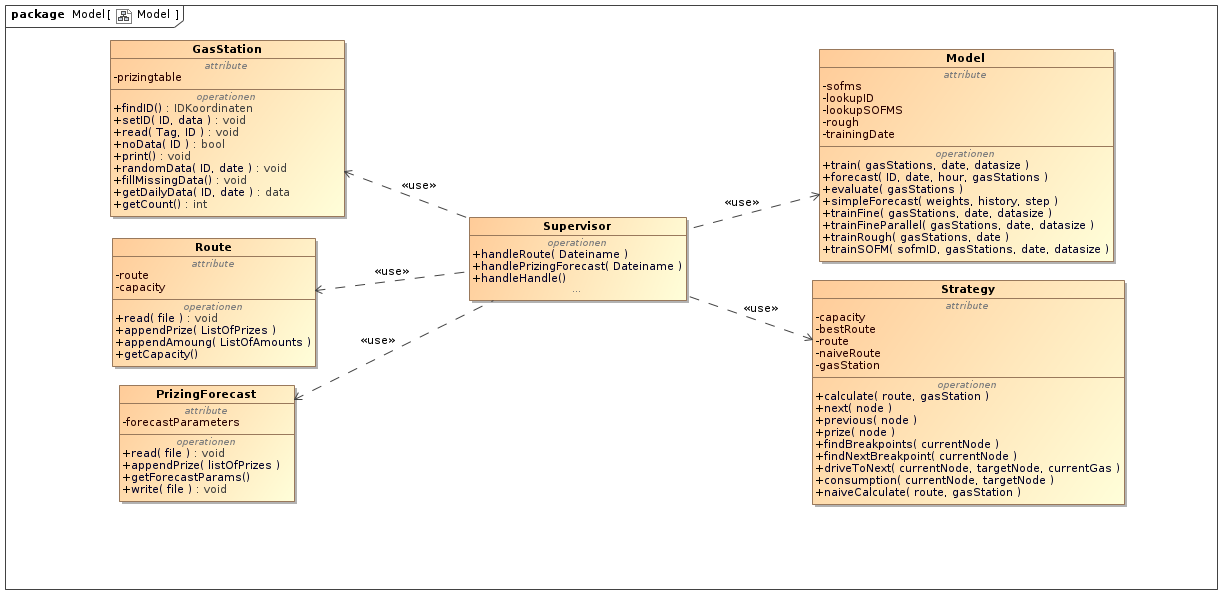
\includegraphics[width=\textwidth]{Model.png}
		\caption{Entwurfsklassendiagramm}
		\label{design}
	\end{figure}
\subsection{Input-einlesende Klassen}
	Die folgenden Beschreibungen der Klassen beziehen sich auf die Gruppe der Input-einlesenden Klassen. Sie sorgen für das korrekte der Einlesen der drei verschiedenen Inputfiles.
\subsubsection{Klasse GasStation}
	Diese Klasse verwaltet die Tankstellen. Kern bildet die List \textit{prizingTable}. Diese speichert für alle Tankstellen die Marke, Koordinaten und historischen Preise. Die weiteren Parameter werden nicht aus den Dateien ausgelesen, da sie für unsere Vorhersagestrategie nicht benötigt werden. Tankstellen für die keine Daten vorliegen werden mit der Methode \textit{fillMissingData} gefüllt. Sie erhalten die Daten der nächsten Tankstelle, die über Daten verfügt.\\
	\textit{getDailyData} gibt die Preise des letzten Jahres zurück. Falls nicht so viele Daten verfügbar sind auch weniger. Diese Daten werden für die Einordnung in Äquivalenzklassen benötigt.\\
	Die Methode \textit{randomData} gibt die Preise acht zusammenhängender Tage zurück. Welche Tage es sind wird dabei zufällig entschieden. Diese Methode wird benötigt, um Trainingsdaten für die einzelnen SOFMs zu bekommen.
\subsubsection{Klasse Route}
	Die Klasse \textit{Route} gehört wie auch die Klasse \textit{GasStation} zu der Gruppe der Input-einlesenden Klassen. Dabei ist diese Klasse mit dem Lesen der Beispielrouten betreut und bietet daher für diese Aufgabe eine Schnittstelle über welche die Routen verwaltet werden können. Neben einem Konstruktor verfügt sie über eine \textit{read}-Methode, welche für das eigentliche Einlesen sorgt und dabei die Attribute \textit{capacity} und \textit{route} befüllt. Das Attribut speichert dabei alle verfügbaren Daten in einer Liste von Tupeln, wobei diese die jeweilige Zeit, in unserer Schreibweise, die ID und einen Platz für den Preis an der jeweiligen Tankstelle und die tankende Menge enthält. Die Methoden \textit{appendPrize} und \textit{appendAmount} fügen Listen von Preisen bzw. Tankmengen mit der richtigen Länge und der richtigen Reihenfolge an diese Plätze ein. \\
	Abschließend beschreibend für diese Klasse ist die \textit{write}-Methode, welche die herausgelesene und modifizierte Datenstruktur \textit{route} wieder in eine Datei schreibt.
\subsubsection{Klasse PrizeForecast}
	Die Klasse \textit{PrizeForecast} übernimmt in unserer Umsetzung die Aufgabe des Einlesens der Vorhersage einzelner Preise. Sie hat aufgrund der Ähnlichkeit der Aufgaben ähnliche Funktionalität.\\ So verfügt die Klasse PrizeForecast über das Attribut forecastParams - eine Liste, welche im folgenden mit Werten bestückt wird, und welche die eingelesenen Daten hält. Für das Einlesen selbst ist die Methode \textit{read} zuständig. Diese liest die Datei ein und wendet dabei die Umformungen an, die bereits in \textit{Umformung der Preisvorhersagedaten} beschrieben wurden. Dadurch finden sich in dieser Datenstruktur der Tag, zu welchem die Preise letztmalig noch als bekannt vorausgesetzt werden dürfen, das Datum des gesuchten Preises, die ID der betreffenden Tankstelle und schlie0lich ein Platzhalter für den Preis selbst. Der Preis kann wie auch in der Klasse Route über eine Methode \textit{appendPrize} angefügt werden. Schließlich kann diese Datenstruktur dann über die write-Methode in die Datei geschrieben werden.
\subsection{Klasse Supervisor}
	%Welche Aufgaben hat die Klasse zu erfüllen? Was sind die wichtigsten Funktionen und was tun diese? Wie werden die Datenstrukturen befüllt und warum auf diese Weise?
	Die Klasse \textbf{Supervisor} kümmert sich um die Koordination der einzelnen Klassen und um das Problem die jeweilig zu bedienenden Schnittstellen zu verwalten. So hat die Klasse als Attribut nur ein Objekt der Klasse GasStation, was  wie oben beschrieben für das Einlesen der Tankstellendaten zuständig ist. Da diese sich zur Laufzeit nicht verändern, kann diese statisch angegeben werden. \\
	Zusätzlich verfügt die Klasse über drei weitere Methoden. Die Methode \textit{handleRoute} nimmt als Parameter einen Dateipfad und kümmert sich um zu bedienende Anfragen einer Tankstrategie für eine Route. So wird ein Objekt der Klasse Route und der Klasse Model erstellt und diese mit dem Einlesen der Daten bzw. dem Erstellen des Modells beauftragt. \\
	Anschließend wird der Preis für die gegebenen Zeitpunkte der Zwischenstopps der Route errechnet und an die Datenstruktur der Route über die Methode \textit{appendPrize} angefügt. Nun wird ein Objekt der Klasse Strategy erzeugt, welche sich um die optimale Tankstrategie auf der Route kümmert. Das Ergebnis wird wieder der Datenstruktur zugeführt und in eine neue Datei geschrieben.\\
	Dementsprechend läuft auch die Logik der Methode \textit{handlePrizeForecast} ab, welche sich mit dem Problem der Preisvorhersage beschäftigt. Diese liest über ein Objekt der Klasse \textit{PrizingForecast} die jeweilige Datei ein und erstellt ein Modell. Nun wird dieses Modell für jeden einzelnen Eintrag dieser Vorhersage-Anfrage trainiert und der Wert der Vorhersagen in die Datenstruktur der Klasse \textit{PrizingForecast} geschrieben. Schließlich wird das Ergebnis in eine Datei geschrieben. \\
	Die Methode \textit{handleHandle} verwaltet diese beiden Methoden und kümmert sich darum, dass diese zum richtige Zeitpunkt angewendet werden. Dafür wird eine config-Datei benutzt in die der Nutzer seine Anfragen schreiben kann. Diese Einträge werden ausgewertet und der jeweiligen Methode zugeführt. \\
	Die Klasse Supervisor führt also letztendlich die Funktionalität aller Funktionen zusammen und ist dementsprechend auch die eigentliche Schnittstelle zu Außenwelt.
\subsection{Klasse Model}
	Diese Klasse bildet den Kern unserer Preisvorhersagung. Ein Modell kann über den Konstruktor erstellt und anschließend mit der Methode \textit{train} trainiert werden. Diese ruft zunächst \textit{trainRough} auf, um die Tankstellen in Äquivalenzklassen einzuordnen und danach werden wird für jede SOFM die Methode \textit{trainSOFM} aufgerufen. Diese aufrufe geschehen entweder sequenziell oder parallel. Standardmäßig wird parallel trainiert mit der Methode \textit{trainFineParallel}.\\
	Nachdem das Modell trainiert wurde kann mit Hilfe der Methode \textit{forecast} der Preis für einen Zeitpunkt in der Zukunft vorhergesagt werden. Die Methode ruft dazu mehrfach \textit{simpleForecast} auf, welche die Preise des nächsten Tages voraussagt.\\
	Des weiteren verfügt die Klasse über eine \textit{evaluate}-Methode. Diese wurde verwendet, um die Güte der Vorhersagen enzuschätzen (siehe Abbildung \ref{Median})
\subsection{Klasse Strategy}
	%Welche Aufgaben hat die Klasse zu erfüllen? Was sind die wichtigsten Methoden und was tun diese? Wie werden die Datenstrukturen befüllt und warum auf diese Weise?
	Die Klasse \textit{Strategy} übernimmt in unserer Anwendung die Umsetzung der oben beschriebenen Lösung des Routenproblems und ist damit essentiell für die Funktionalität. \\
	Die Klasse verfügt dabei über die Schnittstelle \textit{calculate}, welche den oben beschriebenen Algorithmus einleitet und diesen verwaltet. So hat sie dafür die Attribute \textit{capacity} und \textit{route} aus dem Parameter, welcher ein Objekt der Klasse \textit{Route} ist, \textit{gasStation} aus dem Parameter der Methode und \textit{bestRoute} zum schließlichen Halten des Ergebnis der Berechnung. \\
	Die Methoden anderen Methoden sind nur für die Funktionalität dieser Methode angedacht. So setzen \textit{next}, \textit{previous}, \textit{findBreakpoints} und \textit{driveToNext} die Funktionen aus dem oben beschriebenen Algorithmus um. \textit{findNextBreakpoint} ist dabei eine Spezifizierung und dient dem Finden des nächsten Breakpoints auf der Route. Durch die Linearität des Graphen wird hier nur in der Position in der Liste der anzufahrenden Tankstellen gerechnet, was die Berechnung innerhalb der Umsetzung deutlich vereinfacht. Für die Funktionalität ebenfalls wichtig sind die Funktionen \textit{consumption} und \textit{prize}. Letztere errechnet aus einem gegebenen Knoten, der nur als Position in der Liste gegeben ist, den vorher in die Route eingetragenen Preis aus eben jener. \textit{consumption} ist zuständig für die Entfernungsberechnung zwischen zwei Tankstellen. Dieses Problem wird dabei wie in \textbf{Umsetzung der Lösung} des Routenproblems beschrieben, rekursiv gelöst. Es wird also immer der die Entfernung zum nächsten Knoten über die inneren Funktionen der Methode \textit{distance} und deren inneren Funktionen \textit{lat} und \textit{lon}, und \textit{getIDfromPosInRoute} berechnet. Die Funktion dieser Funktionen ist sehr gut dem Identifikator dieser zu entnehmen. \\
	Neben der optimalen Tankstrategie ist hier auch die \glqq naive\grqq{} Tankstrategie wie gefordert in der Methode \textit{naiveCalculate} mit dem eigenen Attribut \textit{naiveRoute} implementiert. Sie greift dabei auf die in der Aufgabenstellung beschriebene Taktik zurück an jeder Tankstelle voll aufzutanken. Die Logik dieser Methode ist entsprechend einfacher. 

\section{Ausblick}
	Das beschriebene Verfahren eignet sich gut, um Benzinpreise vorher zu sagen. Daher lässt es sich natürlich auch genau so auf die Preise für andere Kraftstoffe wie Diesel oder Erdgas übertragen. Für Elektroautos hingegen ist diese Software nicht geeignet: Zum einen schwankt der Strompreis bei weitem nicht so stark wie der Preis für Mineralöl. Solch eine Vorhersage ist also gar nicht notwendig, da die Preise an allen Ladesäulen sehr gleich sind. Des weiteren benötigt das Laden eines Elektroautos wesentlich mehr Zeit als das Tanken eines herkömmlichen Autos. Die Annahme, dass das Tanken also gar keine Zeit verbraucht ist damit hinfällig und die Zeitpunkten wann wir die Tankstellen erreichen passen nicht zur Realität.\\
	Erweiterungen und Verbesserungen der Software wurden auf Seite \pageref{potential} diskutiert.
	
	
	\begin{thebibliography}{999}
		\bibitem {SOFM} Wikipedia, Die freie Enzyklopädie (Hrsg.): Selbstorganisierende Karte; \url{https://de.wikipedia.org/w/index.php?title=Selbstorganisierende_Karte&oldid=172760713}, Zugriff 20.01.2018
		\bibitem {neupy} Yurii Shevchuk: NeuPy Home; \url{http://neupy.com/pages/home.html}, Zugriff 20.01.2018
		\bibitem{routefinding} S. Khuller, A. Malekian und J. án Mestre: Fill or not to Fill: The Gas Station Problem; \url{http://www.cs.umd.edu/projects/gas/gas-station.pdf},  Zugriff 20.01.2018
	\end{thebibliography}
	
\end{document}


